\label{sec: Code}

Simple econometric models can be estimated in a reasonable amount of time on even very modest computers, but as complexity grows estimation becomes increasingly challenging. While there are optimization routines that can optimize the CNL likelihood in reasonable time, implementing these routines is beyond the scope of this paper. For properly efficient estimation the only real option is one of the two specialized tools \textit{Biogeme} and \textit{Larch}. In all of the following we restrict one parameter in each nest to it's true value before estimation, we also assume $\alpha$ and $\mu_m$'s to be fixed at their true values.
\\ \\
We implement reasonably fast versions of the probability equations in \ref{eq: likelihoodderiv}, as well as implementations of $P(m|C)$ and $P(i|m)$ using Numpy in python 3.6. Evaluating the likelihood function in a single point takes approximately 6-7 seconds when using 1.000 observations. As the number of observations increase this process slows further as evident in table \ref{tab: loglikspeed}. This is a major obstacle for estimation, as the large number of parameters, and the complicated effects from parameters on the likelihood, means many observations are generally required to get accurate results.  Optimizing the $J\times K$ parameters jointly fails to converge when using the standard SciPy minimization routine. We do show some results from joint estimation, but one should note that these are from non-converging optimizers.

\begin{center}
\begin{threeparttable}
  \centering
  \caption{Speed comparison five evaluations of $\log\mathcal{L}_K$ at different data sizes}
  \label{tab: loglikspeed}
  \begin{tabular}{lrrrrr}
\toprule
{} &  Obs=10 &  Obs=50 &  Obs=100 &  Obs=1000 &  Obs=5000 \\
\midrule
0 &     1.0 &    5.02 &    10.23 &    124.15 &   1497.02 \\
\bottomrule
\end{tabular}

  \begin{tablenotes}\footnotesize
     \item Numbers are summed time over five iterations of $\log\mathcal{L}_K(\beta, \Theta; x)$ over the dataset with $\alpha$ set to the CNL structure and $\beta$ as described. Units is the running time relative the running time of the $K=10$ dataset. The running time when $Obs=10$ is approximately $0.35$ seconds.
  \end{tablenotes}
\end{threeparttable}
\end{center}

In the following we attempt to estimate model parameters in the CNL model through two very weak, but conceptually simple mechanisms. Especially the first attempt is very unlikely to produce unbiased estimates, let alone estimates that converge. The purpose of showing these attempts should thus not be seen as trying to argue that these methods are in general useable, but to explore the options for estimation in models which are so complex it requires specialist knowledge to code up estimators.

\subsection{Iterative estimation} \label{sec: iteropt}
The perhaps simplest way of estimating the model parameters is the following scheme. We assume that both $\alpha$'s, $\mu$ and $\mu_m$ are known and fixed to their true value. Recall that there is a $\beta$ for each $x$ for every choice (with some set to $0$), so we can arrange $\beta$ as a matrix of size $J\times K$.

\renewcommand{\kbldelim}{(}% Left delimiter
\renewcommand{\kbrdelim}{)}% Right delimiter
\begin{equation} \label{eq:matrices}
  \beta =
  \kbordermatrix{
    & \bm{\beta_0} & \bm{\beta_1} \\
    n_1 & \beta_{00} & \beta_{01} \\
    n_2 & \beta_{10} & \beta_{11} \\
    c_1 & \beta_{20} & \beta_{21} \\
    c_2 & \beta_{30} & \beta_{31} \\
    c_3 & \beta_{40} & \beta_{41} \\
  }
\hookrightarrow
  \kbordermatrix{
    & \bm{\beta_0} & \bm{\beta_1} \\
    n_1 & \beta_{00}^* & \beta_{01}^* \\
    n_2 & \beta_{10}^* & \beta_{11} \\
    c_1 & \beta_{20}^* & \beta_{21} \\
    c_2 & \beta_{30}^* & \beta_{31}^* \\
    c_3 & \beta_{40}^* & \beta_{41} \\
  }
\end{equation}

Our iterative optimization scheme then initialized $\beta^{\textrm{init}} = \bm{\beta^*}$, sets $\beta^{\textrm{init}}_{i0}$ to one as initial value, except for the parameters of choices $c_0$ (which is structural) and $c_3$ which are set to their true values. This is in accordance with the identification stategies outlines in section \ref{sec: Estimation} and illustrated by the right hook arrow in equation \eqref{eq:matrices}. Even though this significantly reduces the number of parameters the Scipy minimizer is still not able to converge when maximizing the likelihood w.r.t the full set of free parameters. We then iteratively optimize each element of $\beta$ assuming all other elements fixed. After each iteration $\beta$ is updated to include the found optimal value. This process is then carried out in a loop until the change in the entire $\beta$ matrix from $t$ to $t+1$ is sufficiently small. In pseudocode a single iteration over the matrix would look like

\begin{algorithm}[H]
  \label{algo:iteroptimizer}
  \SetKwInput{Precondition}{Precondition~}
  \SetKwInput{Input}{Input~}
  \SetKwInput{Data}{Data~}
  \SetKw{Continue}{continue}
  \SetKw{In}{in}

  \caption{Iterative Optimizer}

  \footnotesize
  \DontPrintSemicolon
  \Input{\texttt{$\beta$}: A matrix of parameter vectors}
  \Input{\texttt{$C$}: A vector of choice indices}
  \ForEach{parameter $\beta_i$ \In $\beta$}{
    \ForEach{ choice $c_i$ \In $C$}{
      $\beta_{[b][c]}^*$ = \texttt{OptimizeScalar}($\log\mathcal{L}^{i|\mathcal{C}}_K(\beta, x, \Theta)$) w.r.t $\beta_{[b][c]}$ \\
      $\beta_{[b][c]} \leftarrow \beta_{[b][c]}^*$
    }
  }
\end{algorithm}

As mentioned this process is carried out repeatedly over the continuously updating matrix. Of course this estimation approach is not ideal, but computationally it is feasible to implement within the scope of this paper. For each iteration over the matrix we update the parameter space to be searched, to a slightly narrower segment recentered around the current value of $\beta_{[b][c]}$.

\begin{figure}[h]
  \centering
  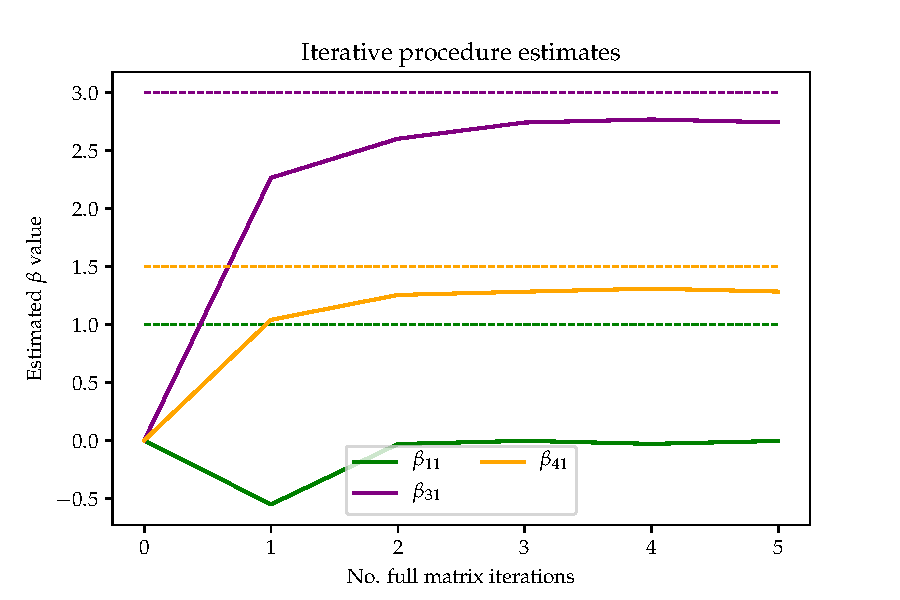
\includegraphics[width=0.8\linewidth]{03_figures/iterEstimate.pdf}
  \caption[Parameter development using iteration.]{Parameter development using iteration. Dashed lines are true parameter values. Each step on the first axis corresponds to a full loop of algorithm \ref{algo:iteroptimizer} over the $\beta$-matrix.}
  \label{fig: iterbetas}
\end{figure}

An intuitive argument for why this method will at least in some cases converge is that if each single-dimensional optimization moves the estimated $\beta$ closer to it's true value, it improves the conditions for estimating the other $\beta$'s in the following iteration bringing them closer to their optimum as well. Thus in the end parameters should converge on their true values. For this to be the case it is essential that the sub-routines consequently move estimates closer to their true values, which will only be the case if the likelihood function is dimensionwise concave, as it is otherwise possible for estimates to move away from their true values in the subroutines. More formally if $\mathcal{L} : \mathbb{R}^n \rightarrow \mathbb{R}$ is a likelihood function dependent on $n$ parameters $\beta$, then if every cross-section of $\ell = \mathcal{L}(\beta_i | \beta_{-i}, \Theta, x)$, $\ell : \mathbb{R} \rightarrow \mathbb{R}$  has a single optimum (implying the function is strictly concave for some sign) and the full function $\mathcal{L}$ has a single optimum as well, then the optima found in $\ell$ after each iteration will converge to the global optimum. This is because 1) the optima in $\ell$ cannot be lower than the global optimum in $\mathcal{L}$, 2) there must be at least one dimension in which a non-global optimum is deviated from (otherwise the function would have local optima) and 3) this deviation will always happen in the direction of the global optimum, as otherwise it would constitute a local optimum. On the other hand in the absence of these rather strict requirements for $\mathcal{L}$ it is intuitive that this kind of optimization will fail.

From figure \ref{fig: iterbetas} it is clear that this simple method suffers from a variety of biases and divergence issues. However this was to be expected. The quick stabilization of estimates might be a sign that the algorithm very quickly approaches a local minimum, which works as an attractor, preventing convergence to the true value. A more formal proof that this is not purely coincidental is needed, but our preliminary testing does provide some circumstantial evidence of (biased) convergence.


\subsection{Joint and nest based optimization}
As an alternative to the naive method implemented above we also attempt a nest based solution, in which we formulate a likelihood based on $\textrm{Pr}(i|m)$ instead of using $\textrm{Pr}(i|C)$ as above. This is in essence the same as considering each choice as it's own $\alpha$-augmented multinomial trial, and therefore requires information on the structural choices. Like with the iterative optimizer this approach is not ideal as coefficients are not restricted across nests, meaning we can get different $\beta$ estimates for cross nested choices, depending on the step of the optimization problem. In exchange the likelihood is significantly simpler, meaning estimation can happen in feasible time.

\begin{figure}[h]
  \centering
  \includegraphics[width=0.8\linewidth]{03_figures/jointEstimation.pdf}
  \caption[Estimate deviations $\beta^* - \hat{\beta}$]{Estimate deviations $\beta^* - \hat{\beta}$ for the nest-based optimization, as well as a joint estimation using the full likelihood.}
  \label{fig: nestandjoint}
\end{figure}

Figure \ref{fig: nestandjoint} show parameters in deviations from their true values when applying the nest-based optimization, as well as (non-convergent) optimization results from attempting to optimize the full likelihood. In both cases we implement the same parameter restrictions as in section \ref{sec: iteropt} for comparison. We take the results as yet another indication that these iterative optimizers are not ideal, but also note that even though the build in Scipy optimizer fails to converge, the results it find are not far from the true values of $\beta$. Actually the Scipy optimizer seems to be about as accurate as our iterative procedure, and the nest based method good only for some parameters. Thus slight improvements in the code might provide good estimates, granted the right parameter restrictions are implemented for identification.

\subsection{Marginal effects in simulated data}
Marginal effects are usually studied in relation to the regressors - that is the question is, if we alter a specific independent variable slightly, what will the resulting change in choice probabilities be. Small changes in specific $\beta$'s are however perhaps even more interesting in a simulation setting, as it is the parameters that vary across choices in the multinomial CNL model. Panel (a) in \ref{fig: marginalities} show for each of 1000 simulated individuals their probability of choosing the cross nested alternative $c_3$ as the $\beta$'s related to the structural nodes $n_1$ and $n_2$ are varied (left and right column respectively). These naturally vary between individuals as the $x$-value is specific to them, meaning a change in $\beta$ affects them differently. The apparent diversity in these curves for different values of $\beta$ is due to the complex changes in $P(i|\mathcal{C})$ when $x$ is either positive or negative, as well as the changes occurring when $|x|\lessgtr 1$.

\begin{figure}[h]
  \begin{center}
  \begin{subfigure}{0.45\linewidth}
    \centering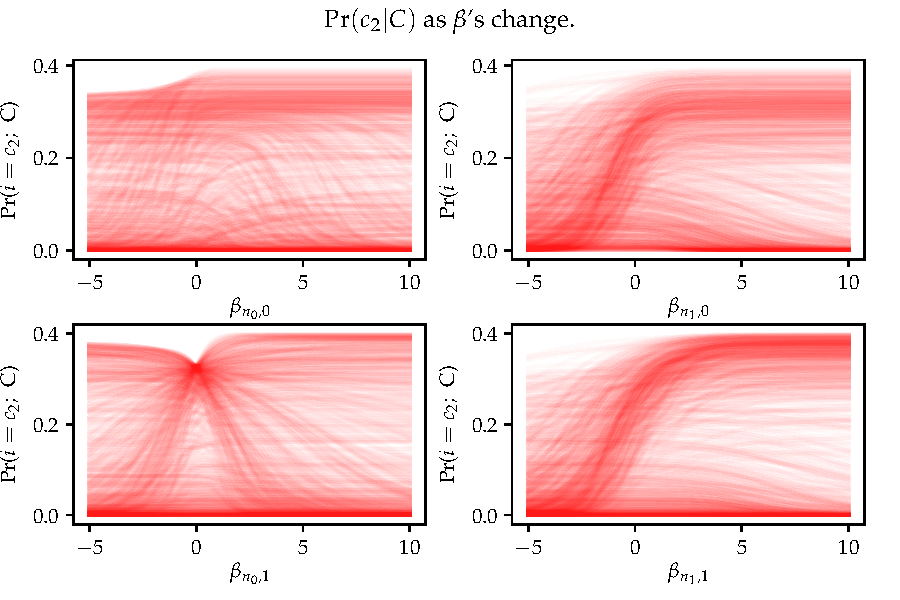
\includegraphics[width=\linewidth]{03_figures/beta_effect.pdf}
    \caption{Individual probabilities as function of $\beta$'s}
  \end{subfigure}
  \begin{subfigure}{0.45\linewidth}
    \centering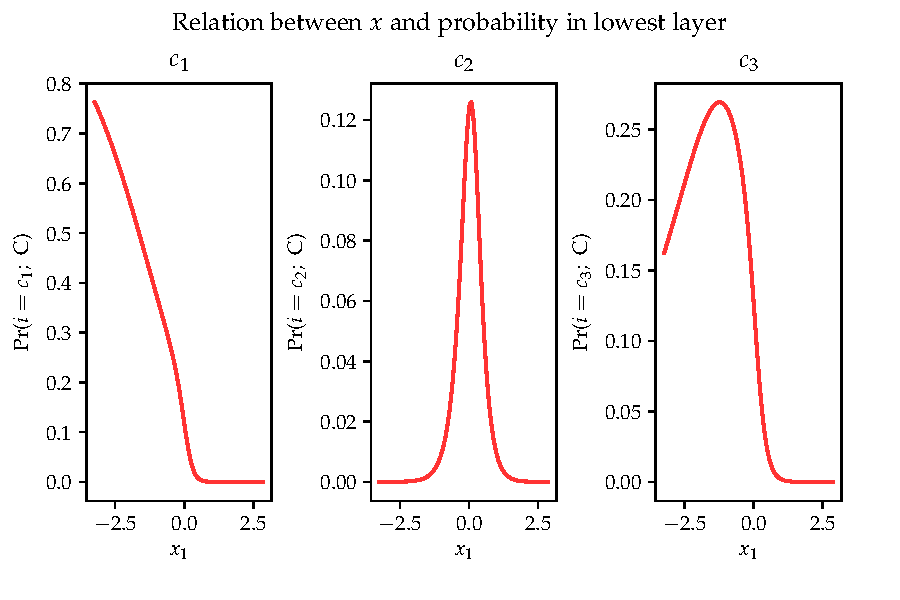
\includegraphics[width=\linewidth]{03_figures/marginaleffects.pdf}
    \caption{Population effects of altering $x_1$ by a constant}
  \end{subfigure}
  \caption{Variations in $P(i|\mathcal{C})$ when altering $\beta$'s and $x$'s}
  \label{fig: marginalities}
\end{center}
\end{figure}

The right panel on the other hand shows choice probabilities as a function of data, specifically $x_1$. These probabilities are naturally identical across the population for a given $x$. The normally considered marginal effects, $\partial p_i / \partial x_i$ is the derivative of these curves. Figure \ref{afig: nl_marginalities} show a plot similar to the one in figure \ref{fig: marginalities} panel (b), but calculated in the nested logit depicted in figure \ref{fig: simpletree}.
\\ \\
Naturally there are many more cross-effects than those shown here. These can easily be constructed by refering to the supplied code.\footnote{The code will be made available on \url{https://github.com/Kristianuruplarsen} after the paper has been graded.} Figure \ref{afig: marginalities} show similar figures but for $\textrm{Pr}(i|m)$, this shows clearly how when conditioning on the specific nest, the probability of making any of the choices are essentially inversely related as in the regular logit.
